\subsection{The {\tt ROD:} module}\label{sect:RODData}

The \moc{ROD:} module used for rod insertion gestion in PWR. This module creates a 3-D field for rod parameter in a fuel map. This local field contains, for each mesh, one coefficient describing the rod insertion for the considered mesh. These coefficients are chosen according to rod coefficients saved in the {\sc saphyb} or {\sc multicompo} object.\\

The \moc{ROD:} module specifications are:

\begin{DataStructure}{Structure \moc{ROD:}}
\dusa{FLMAP} \moc{:=} \moc{ROD:} \dusa{FLMAP} \moc{::} \dstr{descrod1}
\end{DataStructure}

\noindent where
\begin{ListeDeDescription}{mmmmmmmm}

\item[\dusa{FLMAP}] \texttt{character*12} name of the \dds{MAP} object that will contain the 3-D rod file. The \dusa{FLMAP} has to be modified for the module and must appear on both LHS and RHS.

\item[\dstr{descrod1}] structure describing the main input data to the \moc{ROD:} module. Note that this input data is mandatory and must be specified.

\end{ListeDeDescription}

\subsubsection{Main input data to the \moc{ROD:} module}\label{sect:rodmain}

A {\sl rod identification number} (RIN) is a local parameter (type real) assigned to each type of rod in the {\sc saphyb} or
{\sc multicompo} object. Black bars of 900 MW PWRs in France are made of AICN material (Silver-Indium-Cadmium). Black bars of 1300 MW, N4 and EPR  PWRs in France are made of a section of B4C followed by a section of AICN (in yellow), as depicted in Fig.~\ref{fig:rod_pwr}. 

\begin{figure}[h!]
  \begin{center}
    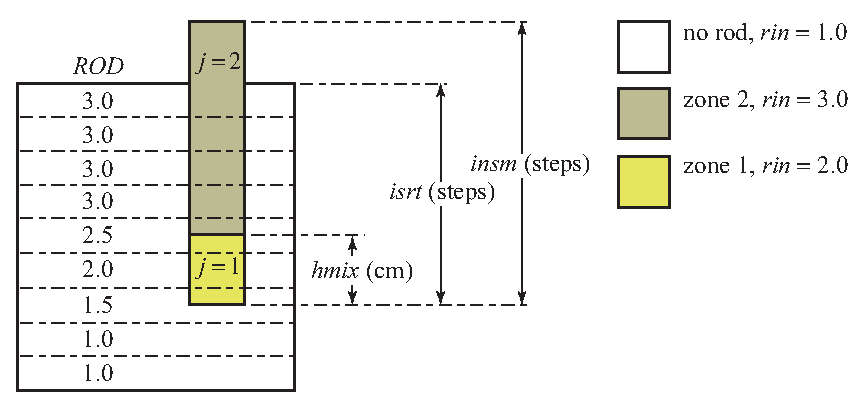
\includegraphics[scale=0.8]{Figures/rod_pwr.eps} 
\caption{Presentation of a partially-inserted 2-part control rod.}\label{fig:rod_pwr}
  \end{center}
\end{figure}

Recommended values are:

\vskip 0.2cm
\begin{tabular}{|c|l|}
\hline
RIN & type of bar \\
\hline
0 & AICG (grey bar, generally out at nominal power) \\
1 ($=$ \dusa{val1}) & rod extracted \\
2 & AICN (black bar, generally out or partly inserted) \\
3 & B4C (black bar, generally out or partly inserted) \\
\hline
\end{tabular}
\vskip 0.2cm

The rod identification number is interpolated over each axial mesh of the fuel map. A local parameter name \dusa{par1} is defined and their distributed values are computed by the {\tt ROD:} module as depicted in Fig.~\ref{fig:rod_pwr}. Local parameters \dusa{par1} are identified as {\sl ROD} in the figure. A local value of {\sl ROD} $=2.5$ corresponds to a mesh of the fuel map containing 50\% of AICN material and 50\% of B4C material.

\noindent

\begin{DataStructure}{Structure \dstr{descrod1}}
$[$ \moc{EDIT} \dusa{iprint} $]$\\
$[$ \moc{PARA} \dusa{par1} \dusa{val1} $]$ \\
$[$ \moc{LINS} \dusa{insm} $]$\\
$[$ \moc{STEP} \dusa{step} $]$\\
$[$ \moc{NRFB} \dusa{nrfb} $]$\\
$[$ \moc{RGRP} \\ 
~~~$\{$ \dusa{ngrp} \dusa{maxmix} \\
~~~~~ ((\dusa{hgrp}(i) \dusa{isrt(i)} \dusa{rin(i,1)} $[[$ \dusa{hmix}(i,j) \dusa{rin(i,j+1)} $]]$), i=1, \dusa{ngrp}, j=1, \dusa{lmix}-1) \\
~~~$|$ \dusa{nrmv} \\
~~~~~ ((\dusa{hgrp}(i) \dusa{isrt(i)}), i=1, \dusa{nrmv}) $\}$ \\
\moc{ENDRGRP} $]$\\
$[$ \moc{RMAP} \dusa{nass} \\
~~~ ((\dusa{hrod}(i,j)), i=1, \dusa{lx}, j=1,ly ) \\
\moc{ENDRMAP} $]$ \\
\moc{;}
\end{DataStructure}

\goodbreak

\noindent where

\begin{ListeDeDescription}{mmmmmmmm}

\item[\moc{EDIT}] keyword used to set \dusa{iprint}.

\item[\dusa{iprint}] integer index used to control the printing on screen:
 = 0 for no print; = 1 for minimum printing (default value); larger values
produce increasing amounts of output.

\item[\moc{PARA}] keyword used to indicate that the name of the record to be
contained the rod field will follow.

\item[\dusa{par1}] name of the rod record and local parameter to be created. This name must correspond to the rod name of the {\sc saphyb} or {\sc multicompo} object.

\item[\dusa{val1}] real value of the 3-D rod field \dusa{par1}. This value enables to initialise the field to a uniform value, corresponding to a core with no rod inserted.

\item[\moc{LINS}] keyword used to indicate the maximum number of insertion steps 
for all rods.

\item[\dusa{insm}] integer value of maximum rod insertion step.

\item[\moc{STEP}] keyword used to indicate the length of one rod step.

\item[\dusa{step}] real value of rod step length (in cm).

\item[\moc{NRFB}] keyword used to indicate the number of bottom-reflective meshes
in the core.

\item[\dusa{nrfb}] integer value of bottom-reflective meshes in the core.

\item[\moc{RGRP}] keyword used to define all rod groups present in the core.

\item[\dusa{ngrp}] integer value of the number of rod groups present in the core.

\item[\dusa{maxmix}] integer value of the maximum number of rod zones (for hybrid 
rods with many materials).

\item[\dusa{nrmv}] integer value of the number of rod groups that rod insertion is modified.

\item[\dusa{hgrp}] \texttt{character*3} identification value for the rod group $i$.

\item[\dusa{isrt}] integer value for the number of inserted steps for the rod group $i$.

\item[\dusa{rin}] real value for the rod identification number (RIN) considered from the {\sc saphyb} or {\sc multicompo} object.

\item[\dusa{hmix}] real value for the height (in cm) of the RIN considered.
If only one RIN is used to define the rod, \dusa{hmix} is not defined. If two or more RIN are used for one rod, 
the values of the lower rod sections with $1\le j < \dusa{lmix}$ should be defined, as depicted in Fig.~\ref{fig:rod_pwr}.

\item[\dusa{lmix}] integer value for the number of \dusa{rin} for each rod group.

\item[\moc{ENDRGRP}] keyword used to indicate the end of rod groups definition.

\item[\moc{RMAP}] keyword used to define the position of each rod group inside the core.

\item[\dusa{nass}] integer value of number of assemblies inside the core.

\item[\dusa{hrod}] \texttt{character*3} identification value for the (i,j) position. Accepted
values are:
\begin{itemize}
\item \moc{|}, \moc{-} or \moc{-|-} for an unrodded assembly,
\item or a \texttt{character*3} identification value referring to the identification value of the rod group.
\end{itemize}

\item[\moc{ENDRMAP}] keyword used to indicate the end of rod group position map.

\end{ListeDeDescription}

\eject
